\documentclass[a5paper]{article}
\usepackage[a5paper, top=8mm, bottom=8mm, left=8mm, right=8mm]{geometry}

\usepackage{polyglossia}
\setdefaultlanguage[babelshorthands=true]{russian}

\usepackage{fontspec}
\setmainfont{FreeSerif}
\newfontfamily{\russianfonttt}[Scale=0.7]{DejaVuSansMono}

\usepackage[font=scriptsize]{caption}

\usepackage{amsmath}
\usepackage{amssymb,amsfonts,textcomp}
\usepackage{color}
\usepackage{array}
\usepackage{hhline}
\usepackage{cite}

\usepackage[hang,multiple]{footmisc}
\renewcommand{\footnotelayout}{\raggedright}

\PassOptionsToPackage{hyphens}{url}\usepackage[xetex,linktocpage=true,plainpages=false,pdfpagelabels=false]{hyperref}
\hypersetup{colorlinks=true, linkcolor=blue, citecolor=blue, filecolor=blue, urlcolor=blue, pdftitle=1, pdfauthor=, pdfsubject=, pdfkeywords=}

\usepackage{tabu}

\usepackage{graphicx}
\usepackage{indentfirst}
\usepackage{multirow}
\usepackage{subfig}
\usepackage{footnote}
\usepackage{minted}

\sloppy
\pagestyle{plain}

\title{ASP.NET, демонстрация}
\author{Юрий Литвинов\\\small{y.litvinov@spbu.ru}}

\date{30.11.2021}

\begin{document}

\maketitle
\thispagestyle{empty}

\section{Введение}

Напишем в качестве демонстрации небольшое приложение, которое позволяет, например, регистрироваться на конференцию (следуя какому-то туториалу, ссылка на который навсегда забыта, впрочем с тех пор всё пару раз полностью переделано). Показывать я буду на примере Visual Studio. Надо, чтобы была установлена <<рабочая нагрузка>> <<ASP.NET и разработка веб-приложений>>.

Для начала требования:

\begin{itemize}
    \item титульная страница конференции со ссылкой на форму регистрации;
    \item форма регистрации, позволяющая зарегистрироваться на конференцию как слушатель или как докладчик --- при регистрации указывается ФИО и почта, и есть чекбокс <<хочу ли выступить с докладом>>.
    \item страница, на которой можно просмотреть всех уже зарегистрировавшихся; поскольку авторизацию мы за пару не сделаем, она будет доступна всем, но ссылки с главной страницы на неё не будет, надо будет заходить по <<правильному>> URL.
\end{itemize}

Из требований понятно, что взаимодействие с пользователем минимально (по сути, просто показать информацию и получить пользовательский ввод), бизнес-логика сводится к работе с базой данных, поэтому выбираем в качестве архитектуры проекта многостраничное приложение на Razor Pages.

\section{Создание проекта}

Начнём с создания нового проекта. Create a new project -> ASP.NET Core Web App (можно облегчить поиск, выбрав в фильтрах сверху C\#, All Platforms, Web). Указываем имя и расположение проекта как обычно (назовём проект ConferenceRegistration), оставляем в следующем окне всё по умолчанию.

Запустим и посмотрим, что получилось. Для этого достаточно просто нажать на <<Запустить>>, но можно посмотреть на кнопку запуска внимательнее и выяснить, что она позволяет выбрать \textit{хостинг} для нашего приложения и браузер, в котором мы хотим наше приложение посмотреть. По умолчанию приложение запускается в self-hosted-режиме --- внутри процесса приложения запускается веб-сервер Kestrel. Можно выбрать IIS Express, а можно WSL (тогда приложение запустится на линуксовой виртуальной машине, тоже в self-hosted-режиме --- это полезно, чтобы более-менее реалистично посмотреть, как оно будет работать в реальном линуксовом окружении, но требует длительной настройки, поэтому мы не будем). 

Приложение запустится в выбранном браузере по адресу localhost (потому что отладочные серверы по умолчанию извне локального компьютера не видны) и случайному порту, определяемому при запуске (впрочем, это можно перенастроить в Properties/launchSettings.json, свойство <<applicationUrl>>). Ещё обратите внимание, что, в отличие от десктопных приложений, закрытие окна браузера не всегда означает остановку приложения, и наоборот, если вы остановите приложение, окно браузера не обязано закрыться --- Visual Studio старается делать это сама, но у неё не всегда получается (в частности, когда в браузере открыто несколько вкладок).

При первом запуске Visual Studio попросит добавить самоподписанный отладочный сертификат в список доверенных, поскольку мы, как все нормальные люди, сразу делаем приложение с поддержкой HTTPS. Соглашаемся. В реальном окружении потребуется настоящий сертификат, но мы не будем на демо этим заморачиваться.

\section{Hello, world}

Начнём с того, что удалим всё содержимое папки Pages, поскольку мы хотим всё сделать своими руками (опять-таки, в реальной жизни сгенерированный шаблон на самом деле может быть полезен). Кликаем правой кнопкой на папку Pages, говорим <<Add Razor Page>>, выбираем <<Razor Page --- Empty>> (это будет главная страница, там ничего интересного не нужно), жмём <<Add>>. Оставляем название по умолчанию <<Index.cshtml>>. Получаем вот такой View:

\begin{minted}{html}
@page
@model ConferenceRegistration.Pages.IndexModel
@{
}
\end{minted}

И вот такой код, его поддерживающий

\begin{minted}{csharp}
using Microsoft.AspNetCore.Mvc;
using Microsoft.AspNetCore.Mvc.RazorPages;

namespace ConferenceRegistration.Pages
{
    public class IndexModel : PageModel
    {
        public void OnGet()
        {
        }
    }
}
\end{minted}

Давайте сразу же перейдём на C\# 10 (если нет желания, можно этого не делать и не сражаться с IDE, где всё ещё старые шаблоны):

\begin{minted}{csharp}
global using Microsoft.AspNetCore.Mvc;
global using Microsoft.AspNetCore.Mvc.RazorPages;
\end{minted}

вставим первыми строчками в Program.cs, а код страницы сделаем с file-scoped namespace:

\begin{minted}{csharp}
namespace ConferenceRegistration.Pages;

public class IndexModel : PageModel
{
    public void OnGet()
    {
    }
}
\end{minted}

Теперь давайте напишем что-нибудь содержательное во View:

\begin{minted}{html}
@page

<!DOCTYPE html>

<html>
    <head>
        <meta name="viewport" content="width=device-width" />
        <title>Hello</title>
    </head>
    <body>
        Hello, world!
    </body>
</html>
\end{minted}

Запускаем, проверяем, что всё работает. И действительно, должна выводиться убогая надпись <<Hello, world!>> в браузере.

\section{Регистрация}

Чтобы написать <<Hello, world!>>, никакого ASP.NET не нужно, это могла бы быть статическая HTML-страница. Давайте пойдём дальше и сделаем форму регистрации. Для этого добавим новую Razor-страницу, Registration.cshtml, тоже типа <<Razor Page --- Empty>> (мы сами потом сможем прикрутить к ней БД). Начнём с моделирования предметной области. Поскольку она предельно проста, мы можем сделать это прямиком в коде поддержки страницы. В более суровых случаях нам надо было бы сделать отдельно доменную модель, отдельно View Model-ы, и держать их отдельно от контроллеров, но в более суровых случаях нам бы потребовались и настоящие контроллеры, и полноценный MVC, и даже отдельный проект с доменной моделью. Но это всё не лезет в ознакомительный кусочек про веб-программирование в этом курсе. Итак:

\begin{minted}{csharp}
namespace ConferenceRegistration.Pages;

[BindProperties]
namespace ConferenceRegistration.Pages;

[BindProperties]
public class RegistrationModel : PageModel
{
    public string Name { get; set; } = "";

    public string Email { get; set; } = "";

    public bool IsSpeaker { get; set; }
}
\end{minted}

Обратите внимание на атрибут \mintinline{csharp}{[BindProperties]} над классом --- он говорит ASP.NET, что при получении запроса с параметрами, совпадающими по именам со свойствами (в нашем случае Name и Email), надо их содержимое положить в соответствующие свойства модели. Теперь у нас RegistrationModel --- это не просто поддерживающий страницу код, а суть доменный класс <<участник конференции>> плюс примешанные к нему средства доставки (наследование от PageModel), а потом ещё тут же будут и средства обеспечения персистентности (работа с базой), что для больших проектов нельзя смешивать, но для маленьких вполне ок.

Ещё обратите внимание на то, что свойства проинициализированы пустыми строками --- в C\# 10 Nullability-анализ включён по умолчанию, так что строки (как ссылочный тип) должны быть не \mintinline{csharp}{null} сразу же. А IsSpeaker имеет тип-значение, поэтому он \mintinline{csharp}{null} и так быть не может.

Теперь добавим HTML-разметку для нашей страницы:

\begin{minted}{html}
@page
@model ConferenceRegistration.Pages.RegistrationModel
@addTagHelper *, Microsoft.AspNetCore.Mvc.TagHelpers

<html>
    <head>
        <meta name="viewport" content="width=device-width" />
        <title>Register</title>
    </head>
    <body>
        <form asp-action="Register" method="post">
            <p>
                <label asp-for="Name">Your name:</label>
                <input asp-for="Name" />
            </p>
            <p>
                <label asp-for="Email">Your email:</label>
                <input asp-for="Email" />
            </p>
            <p>
                <label>Are you a speaker?</label>
                <select asp-for="IsSpeaker">
                    <option value="">Choose an option</option>
                    <option value="true">Yes</option>
                    <option value="false">No</option>
                </select>
            </p>
            <button type="submit">Register!</button>
        </form>
    </body>
</html>
\end{minted}

Тут используются \emph{тэг-хелперы} для описания HTML-формы и её содержимого (про них рассказывалось в предыдущей лекции). Тут тэг-хелперы используются для задания соответствия полей формы и модели (с помощью атрибута asp-for, который заставляет компилятор проверить, что такое свойство у модели действительно есть и правильного типа, и потом ещё отображать результат серверной валидации --- когда мы до неё дойдём).

Уже можно запустить приложение и посмотреть, что получилось. По умолчанию откроется титульная страница, но мы можем вручную перейти на форму регистрации по URL \url{https://localhost:7207/Registration}. Пока что по клику на Submit, впрочем, ничего не произойдёт. Но пока что давайте поправим титульную страницу, чтобы отлаживаться было удобнее:

\begin{minted}{html}
@page

@addTagHelper *, Microsoft.AspNetCore.Mvc.TagHelpers

<html>
    <head>
        <meta name="viewport" content="width=device-width" />
        <title>SEIM-2022 registration</title>
    </head>
    <body>
        <div>
            <p>SEIM-2022 conference will be held in April in St. Petersburg.</p>
            <a asp-page="Registration">Register now!</a>
        </div>
    </body>
</html>
\end{minted}

Это в Index.cshtml. Обратите внимание на атрибут тэг-хелпера asp-page --- он генерирует корректную ссылку на страницу приложения.

Теперь вернёмся к форме регистрации и добавим в Registration.cshtml.cs обработчик POST-запроса, в котором мы скоро будем сохранять в базу присланные данные:

\begin{minted}{csharp}
namespace ConferenceRegistration.Pages;

[BindProperties]
public class RegistrationModel : PageModel
{
    public string Name { get; set; } = "";

    public string Email { get; set; } = "";

    public bool IsSpeaker { get; set; }

    public void OnPost()
    {
        // TODO: Do something with registration info.
    }
}
\end{minted}

И, наконец, перейдём к работе с базой данных.

\section{Персистентность}

\subsection{Модель данных}

Напомним, что хранить данные в памяти в веб-приложениях нельзя, потому что если веб-приложение по тем или иным причинам будет выгружено из памяти, данные потеряются (а для веб-приложений причин может быть масса, и это абсолютно нормально). Так что давайте прикрутим поддержку базы. 

За общение с базой отвечает ORM-система, в .NET это почти всегда Entity Framework Core. EF Core позволяет по уже готовой БД сгенерировать код соответствующих классов, но поскольку модель данных у нас очень простая, а приложение не то чтобы высоконагруженное, мы используем подход Code First --- сначала опишем классы в коде, затем позволим EF Core создать по ним схему БД.

Итак, для начала опишем то, в каком виде мы хотим хранить данные. У нас, вообще говоря, уже есть модель участника конференции, но давайте сделаем по-человечески и вынесем эту модель явно, в отдельный класс. Создадим в корне проекта папку Data, в ней класс Participant, перенесём в него данные из модели:

\begin{minted}{csharp}
namespace ConferenceRegistration.Data;

public class Participant
{
    public string Name { get; set; } = "";

    public string Email { get; set; } = "";

    public bool IsSpeaker { get; set; }
}
\end{minted}

И подправим саму модель, чтобы она работала с этим классом:

\begin{minted}{csharp}
using ConferenceRegistration.Data;

namespace ConferenceRegistration.Pages;

[BindProperties]
public class RegistrationModel : PageModel
{
    public Participant Participant { get; set; } = new();

    public void OnPost()
    {
        // TODO: Do something with registration info.
    }
}
\end{minted}

И представление, чтобы оно знало про отрефакторенную модель:

\begin{minted}{html}
@page

@model ConferenceRegistration.Pages.RegistrationModel

@addTagHelper *, Microsoft.AspNetCore.Mvc.TagHelpers

<html>
    <head>
        <meta name="viewport" content="width=device-width" />
        <title>Register</title>
    </head>
    <body>
        <form asp-action="Register" method="post">
            <p>
                <label asp-for="Participant.Name">Your name:</label>
                <input asp-for="Participant.Name" />
            </p>
            <p>
                <label asp-for="Participant.Email">Your email:</label>
                <input asp-for="Participant.Email" />
            </p>
            <p>
                <label>Are you a speaker?</label>
                <select asp-for="Participant.IsSpeaker">
                    <option value="">Choose an option</option>
                    <option value="true">Yes</option>
                    <option value="false">No</option>
                </select>
            </p>
            <button type="submit">Register!</button>
        </form>
    </body>
</html>
\end{minted}

\subsection{DbContext}

Теперь нам потребуется EF-специфичная штука: DbContext, класс для доступа к базе. Создаём в папке Data класс ConferenceRegistrationDbContext такого содержания:

\begin{minted}{csharp}
using Microsoft.EntityFrameworkCore;

namespace ConferenceRegistration.Data;

public class ConferenceRegistrationDbContext: DbContext
{
    public ConferenceRegistrationDbContext(
        DbContextOptions<ConferenceRegistrationDbContext> options)
        : base(options)
    {
    }

    public DbSet<Participant> Participants => Set<Participant>();
}
\end{minted}

Тут нас в какой-то момент (например, после того, как вы напечатаете DbContext и нажмёте в Visual Studio Ctrl+.) попросят ещё поставить Nuget-пакет Entity Framework Core, соглашайтесь.

Теперь добавим поддержку нашего нового DbContext-а в страницу, используя магию Dependency Injection:

\begin{minted}{csharp}
using ConferenceRegistration.Data;

namespace ConferenceRegistration.Pages;

[BindProperties]
public class RegistrationModel : PageModel
{
    private readonly ConferenceRegistrationDbContext _context;

    public RegistrationModel(ConferenceRegistrationDbContext context)
        => _context = context;

    public Participant Participant { get; set; } = new();

    public async Task<IActionResult> OnPostAsync()
    {
        _context.Participants.Add(Participant);
        await _context.SaveChangesAsync();

        return RedirectToPage("./Index");
    }
}
\end{minted}

Тут мы декларируем, что для работы нашему классу нужен экземпляр ConferenceRegistrationDbContext, который мы принимаем в конструктор и сохраняем себе. Дальше мы переписали OnPost на OnPostAsync, возвращающий Task<IActionResult> --- чтобы иметь возможность отправить на фронт результат действия, в нашем случае это пока будет редирект на начальную страницу.

\subsection{Конфигурирование БД}

Теперь, собственно, конфигурация базы. Поскольку данных немного и нужны они только нашему сервису, воспользуемся локальной базой и СУБД внутри процесса приложения. Хороший вариант для этого --- СУБД SQLite, она не требует установки, подключается как библиотека, хранит данные просто в файле на диске, но вместе с тем поддерживает полноценный SQL и внешне ведёт себя как любая другая реляционная база данных, так что перейти на что-нибудь взрослое можно будет просто заменой конфига (по идее).

Для начала установим Nuget-пакет Microsoft.EntityFrameworkCore.Sqlite. Дальше сконфигурируем в Program.cs базу и добавим её в список сервисов, доступных Dependency Injection:

\begin{minted}{csharp}
global using Microsoft.AspNetCore.Mvc;
global using Microsoft.AspNetCore.Mvc.RazorPages;

using ConferenceRegistration.Data;
using Microsoft.EntityFrameworkCore;

var builder = WebApplication.CreateBuilder(args);

// Add services to the container.
builder.Services.AddRazorPages();

builder.Services.AddDbContext<ConferenceRegistrationDbContext>(options =>
    options.UseSqlite("Data Source=conferenceRegistration.db"));

var app = builder.Build();
\end{minted}

Тут используется connection string, которая говорит, что собственно данные хранятся в файле conferenceRegistration.db, лежащем в рабочей папке приложения. Не делайте так в продакшн-коде --- connection string по-хорошему надо вынести в конфиг, но всему своё время. Метод AddDbContext создаёт экземпляр ConferenceRegistrationDbContext (вызывая тот самый загадочный конструктор с DbContextOptions из примера выше) и запоминает его в DI-контейнере приложения. Теперь, когда ASP.NET будет создавать класс модели страницы, он увидит рефлексией, что ему в конструктор надо передать экземпляр ConferenceRegistrationDbContext и пойдёт искать его в контейнере. Всем остальным страницам, которым нужен доступ к базе, передастся этот же экземпляр, без всяких усилий со стороны разработчика. На самом деле, в DI-контейнере ASP.NET можно регистрировать и свои собственные сервисы, тем самым избегая хлопотного ручного создания объектов и передачи зависимостей туда-сюда (а с учётом того, что в ASP.NET временем жизни классов управляет сам фреймворк, без DI очень просто с ума сойти).

Попробуем это дело запустить (хотя ещё не должно работать, базы-то нет). Пробуем зарегистрироваться, получаем 

\begin{minted}{text}
System.InvalidOperationException: The entity type 'Participant' requires 
    a primary key to be defined.
\end{minted}

Да, нам надо дополнить нашу модель данных реляционными штуками, такими как первичный ключ (поскольку ключ не часть доменной модели, в больших приложениях нам потребуется иметь отдельный набор классов для хранения в базе и отдельный --- для бизнес-логики, которые <<persistense-agnostic>>, чтобы не загромождать доменную модель; но мы тут выпендриваться не будем):

\begin{minted}{csharp}
namespace ConferenceRegistration.Data;

public class Participant
{
    public int ParticipantId { get; set; }

    public string Name { get; set; } = "";

    public string Email { get; set; } = "";

    public bool IsSpeaker { get; set; }
}
\end{minted}

Опять-таки, применяется подход Convention over configuration, так что EF Core сама догадывается, что ParticipantId --- это первичный ключ для будущей таблицы в базе.

\subsection{Миграции}

Запускаем приложение снова, пытаемся зарегистрироваться, и получаем теперь вот такое:

\begin{minted}{text}
SqliteException: SQLite Error 1: 'no such table: Participants'.
\end{minted}

Это потому, что мы всё со стороны приложения сконфигурировали и подготовили, но самой базы пока нет. Открываем HeidiSQL и начинаем вручную создавать схему базы? Нет, EF Core все сделает сама --- мы ведь используем подход Code First, схема БД (из одной таблички) описана у нас в коде в папке Data. Для того, чтобы нам создали базу, надо:

\begin{enumerate}
    \item Поставить инструмент .NET CLI, который называется dotnet-ef. По умолчанию он не установлен, поэтому открываем Package Manager Console (Tools -> NuGet Package Manager -> Package Manager Console) и пишем там \mintinline{text}{dotnet tool install --global dotnet-ef}.
    \item Дальше надо добавить пакет Microsoft.EntityFrameworkCore.Design, можно там же, в консоли: \mintinline{text}{dotnet add package Microsoft.EntityFrameworkCore.Design} (единственное что убедитесь, что команда запускается из директории с .csproj, при необходимости сделайте cd). Это штука, которая поддерживает генерацию \emph{миграций} по коду.
    \item Дальше генерируем \emph{миграцию}: \mintinline{text}{dotnet ef migrations add InitialCreate}. У нас в проекте появилась папка Migrations, в которой есть сгенерированный класс <<InitialCreate>> с методами Up и Down. Up, собственно, создаёт схему БД (используя connection string, который мы сконфигурировали в Program).
    \item И последнее, миграцию надо применить: \mintinline{text}{dotnet ef database update}.
\end{enumerate}

Сгенерированный код миграций коммитится в репозиторий как часть проекта, а вот сама БД --- нет, поэтому последний шаг надо применять после каждого git clone и git clean. Что легко забыть, но ошибка об отсутствии таблицы напомнит.

Теперь запускаем-проверяем, оказывается, что регистрация правда работает теперь, но мы не можем посмотреть, реально ли данные о регистрации записались в базу. Но мы можем открыть базу уже знакомым нам HeidiSQL, просто указав как вид базы SQLite и выбрав путь до файла .db. 

\section{Список участников}

Давайте сделаем отдельную страницу, где показывались бы зарегистрированные участники, чтобы не надо было вручную лезть в базу. Создадим новую Razor Page ListParticipants.cshtml, с вот такой Razor-разметкой:

\begin{minted}{html}
@page

@model ConferenceRegistration.Pages.ListParticipantsModel

<html>
    <head>
        <meta name="viewport" content="width=device-width" />
        <title>ListParticipants</title>
    </head>
    <body>
    <h2>List of conference participants:</h2>
    <table>
        <thead>
            <tr>
                <th>Name</th>
                <th>Email</th>
                <th>Is speaker</th>
            </tr>
        </thead>
        <tbody>
            @foreach (ConferenceRegistration.Data.Participant p in Model.Participants) {
                <tr>
                    <td>@p.Name</td>
                    <td>@p.Email</td>
                    <td>@(p.Speaker ? "Yes" : "No")</td>
                </tr>
            }
        </tbody>
    </table>
    </body>
</html>
\end{minted}

Тут создаётся HTMLная таблица, в которой просто подряд как строки выводятся все зарегистрированные участники из модели. Соответственно, надо создать модель:

\begin{minted}{csharp}
using ConferenceRegistration.Data;

namespace ConferenceRegistration.Pages;

public class ListParticipantsModel : PageModel
{
    private readonly ConferenceRegistrationDbContext context;

    public ListParticipantsModel(ConferenceRegistrationDbContext context)
        => this.context = context;

    public IList<Participant> Participants { get; private set; } = new List<Participant>();

    public void OnGet()
    {
        Participants = context.Participants.OrderBy(p => p.ParticipantId).ToList();
    }
}
\end{minted}

Тут мы, как и раньше, получаем как зависимость контекст базы данных, и просто читаем из него список участников, сортируя по Id-шникам (просто на всякий случай).

Запускаем, идём на \url{https://localhost:порт/ListParticipants}, проверяем, что всё работает.

\section{Страница подтверждения регистрации}

Теперь давайте добавим ещё одну маленькую страницу, которая бы показывалась, когда мы успешно зарегистрировались на конференцию: Thanks.cshtml. View очень простой:

\begin{minted}{html}
@page

@model ConferenceRegistration.Pages.ThanksModel

<html>
    <head>
        <meta name="viewport" content="width=device-width" />
        <title>Thanks</title>
    </head>
    <body>
        <p>
            <h1>Thank you, @Model.Participant.Name</h1>
        </p>
        <p>
            @if (Model.Participant.IsSpeaker)
            {
                @:Please don't forget to submit your article!
            }
        </p>
    </body>
</html>
\end{minted}

И модель: 

\begin{minted}{csharp}
using ConferenceRegistration.Data;

namespace ConferenceRegistration.Pages;

public class ThanksModel : PageModel
{
    public Participant Participant { get; set; } = new();

    public void OnGet(Participant participant)
    {
        Participant = participant;
    }
}
\end{minted}

И теперь надо поправить Registration.cshtml.cs, чтобы она отправляла участника на новую страницу:

\begin{minted}{csharp}
...
public class RegistrationModel : PageModel
{
    ...
    public async Task<IActionResult> OnPostAsync()
    {
        context.Participants.Add(Participant);
        await context.SaveChangesAsync();

        return RedirectToPage("./Thanks", Participant);
    }
}
\end{minted}

Тут используется перегрузка RedirectToPage, принимающая вторым аргументом route values --- значения, которые дописываются как параметр у URL. При редиректе Participant честно сериализуется и мы получаем URL в духе \url{https://localhost:7207/Thanks?ParticipantId=3&Name=yurii&Email=123&IsSpeaker=True}. Что вполне ок для наших целей, но если бы мы хотели, чтобы URL не содержал в себе вообще все данные модели, мы могли бы передавать сюда только id-шник, и грузить Participant из базы. Пытаться как-то по-хитрому передавать данные между страницами, держа их в памяти, в веб-приложениях может быть плохой идеей.

\section{Оформление}

Базовая функциональность готова, теперь можно заняться внешним видом сайта. Сейчас сделано без какого-либо оформления вообще, а так даже школьники нынче не верстают. 

Поэтому воспользуемся одной из библиотек, доступных в проекте <<из коробки>> --- Bootstrap. Это третьесторонняя опенсорсная библиотека 
(\url{http://getbootstrap.com/}), очень известная в мире веб-разработки, она поставляется вместе с ASP.NET и даже включена в стандартный шаблон приложения (версии 5.1, это важно --- в интернетах полно туториалов по более старому Bootstrap, и они не поддерживают обратную совместимость). Bootstrap много чего умеет, но мы воспользуемся некоторыми CSS-стилями, которые она определяет. Например, модифицируем
стартовую страницу так:

\begin{minted}{html}
@page

@addTagHelper *, Microsoft.AspNetCore.Mvc.TagHelpers

<html>
    <head>
        <meta name="viewport" content="width=device-width" />
        <title>SEIM-2022 registration</title>
        <link rel="stylesheet" href="/lib/bootstrap/dist/css/bootstrap.css" />
    </head>
    <body>
        <div class="text-center">
            <h3>SEIM-2022 conference will be held in April in St. Petersburg.</h3>
            <a class="btn btn-primary" asp-page="Registration">Register now!</a>
        </div>
    </body>
</html>
\end{minted}

Добавилось подключение bootstrap.css, атрибуты class="text-center" и class="btn btn-primary", ещё по мелочи изменено внешнее представление. Если сейчас запустить приложение, будет видно, что стало лучше (не то чтобы сильно лучше, но верстаем как можем).

Форма регистрации:

\begin{minted}{html}
@page

@model ConferenceRegistration.Pages.RegistrationModel

@addTagHelper *, Microsoft.AspNetCore.Mvc.TagHelpers

<html>
    <head>
        <meta name="viewport" content="width=device-width" />
        <title>Register</title>
        <link rel="stylesheet" href="/lib/bootstrap/dist/css/bootstrap.css" />
    </head>
    <body>
        <div class="row mb-3 text-center"><h4 class="col-sm-6">Registration form</h4></div>
        <form asp-action="Register" method="post">
            <div class="row mb-3">
                <label class="col-sm-1 col-form-label col-form-label-lg" 
                    asp-for="Participant.Name">Your name:</label>
                <div class="col-sm-4">
                    <input class="form-control form-control-lg" 
                        asp-for="Participant.Name" />
                </div>
            </div>
            <div class="row mb-3">
                <label class="col-sm-1 col-form-label col-form-label-lg" 
                    asp-for="Participant.Email">Your email:</label>
                <div class="col-sm-4">
                    <input class="form-control form-control-lg" 
                        asp-for="Participant.Email" />
                </div>
            </div>
            <div class="row mb-3">
                <label class="col-sm-1 col-form-label col-form-label-lg">
                    Are you a speaker?
                </label>
                <div class="col-sm-4">
                    <select class="form-select form-select-lg" 
                        asp-for="Participant.IsSpeaker">
                        <option value="">Choose an option</option>
                        <option value="true">Yes</option>
                        <option value="false">No</option>
                    </select>
                </div>
            </div>
            <div class="row mb-3 mx-auto">
                <div class="col-sm-5 d-grid gap-2">
                    <button class="btn btn-primary btn-lg" type="submit">
                        Register!
                    </button>
                </div>
            </div>
        </form>
    </body>
</html>
\end{minted}

Каждому контролу на форме добавились атрибуты управления лейаутом (col-что-то-размер), form-label и form-control, и несколько новых div-ов, чтобы повесить на них классы, которые bootstrap будет использовать, чтобы применить стили. Запускаем-проверяем, должно было получиться что-то такое:

\begin{center}
    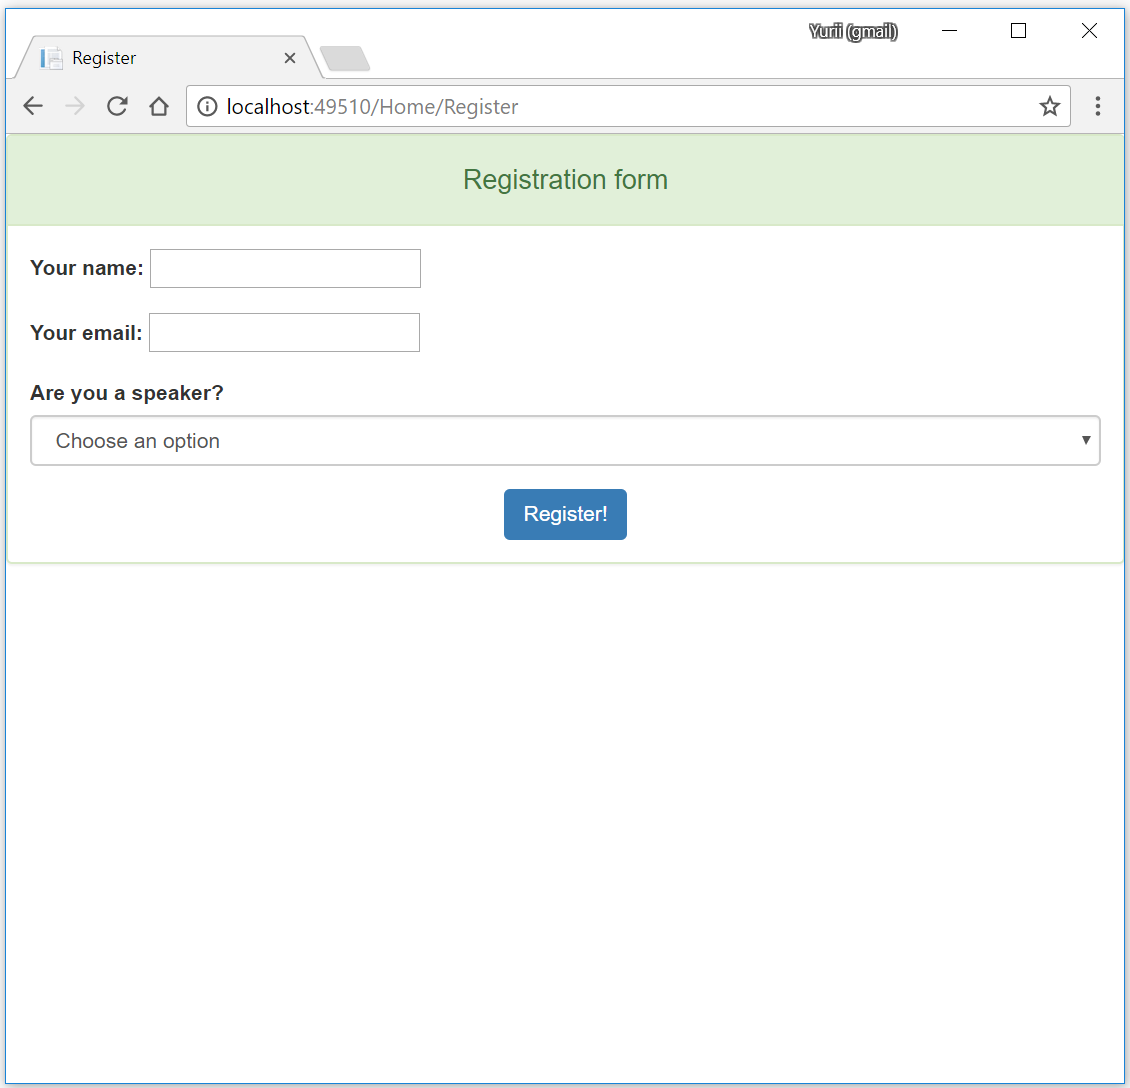
\includegraphics[width=0.55\textwidth]{styledRegisterForm.png}
\end{center}

В целом, наверное, неплохо выглядит на мобильниках. Теперь займёмся страницей со списком участников:

\begin{minted}{html}
@page

@model ConferenceRegistration.Pages.ListParticipantsModel

<html>
    <head>
        <meta name="viewport" content="width=device-width" />
        <title>ListParticipants</title>
        <link rel="stylesheet" href="/lib/bootstrap/dist/css/bootstrap.css" />
    </head>
    <body>
        <div class="row mb-3 text-center">
            <h2 class="col-sm-6">List of conference participants</h2>
        </div>
        <table class="table table-striped table-bordered">
            <thead>
            <tr>
                <th>Name</th>
                <th>Email</th>
                <th>Is speaker</th>
            </tr>
            </thead>
            <tbody>
            @foreach (ConferenceRegistration.Data.Participant p in Model.Participants) {
                <tr>
                    <td>@p.Name</td>
                    <td>@p.Email</td>
                    <td>@(p.IsSpeaker ? "Yes" : "No")</td>
                </tr>
            }
            </tbody>
        </table>
    </body>
</html>
\end{minted}

Должно было получиться что-то такое:

\begin{center}
    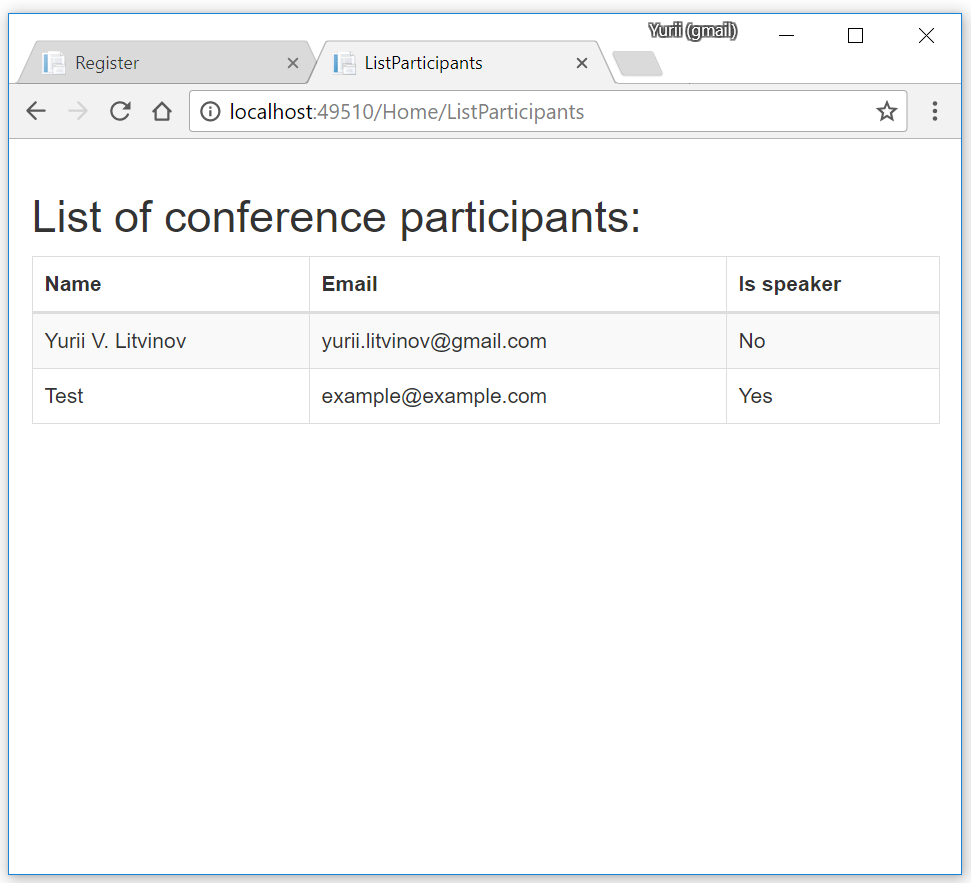
\includegraphics[width=0.55\textwidth]{styledListParticipants.png}
\end{center}

Выглядит это всё как написание каких-то заклинаний, но на самом деле на сайте Bootstrap есть подробная документация с примерами, так что найти нужные классы несложно. Сложно на самом деле придумать и придерживаться какого-то стандарта по вёрстке, как пример такого стандарта мору рекомендовать \url{https://guides.kontur.ru/}.

Оформление страницы с подтверждением регистрации оставляется как упражнение.

\section{Валидация}

Сейчас зарегистрироваться на конференцию можно, просто тыкнув на Register и ничего не вводя. Давайте добавим валидацию, благо это совсем несложно. Просто модифицируем модель Participant в папке Data:

\begin{minted}{csharp}
using System.ComponentModel.DataAnnotations;

namespace ConferenceRegistration.Data;

public class Participant
{
    [Required(ErrorMessage = "Please enter your name")]
    public string Name { get; set; }

    [Required(ErrorMessage = "Please enter your email")]
    [RegularExpression(".+\\@.+\\..+", ErrorMessage = "Please enter a valid email address")]
    public string Email { get; set; }

    [Required(ErrorMessage = "Please specify whether you'll be a speaker or just attending")]
    public bool? Speaker { get; set; }
}
\end{minted}

Так выглядит декларативное описание правил корректности данных в модели, которое ASP.NET будет применять каждый раз, когда делает model binding при приёме запроса. Кстати, обратите внимание, мы специально сделали Speaker nullable, так что если пользователь ничего не ввёл, там будет null. Из-за этого нам теперь надо найти все \mintinline{csharp}{if (IsSpeaker)} и заменить на \mintinline{csharp}{if (IsSpeaker == true)}, но оно того стоит.

Само по себе оно ничего интересного не делает, кроме выставления флага IsValid в поле ModelState модели страницы, поэтому надо ещё модифицировать модель:

\begin{minted}{csharp}
...
public class RegistrationModel : PageModel
{
    ...
    public async Task<IActionResult> OnPostAsync()
    {
        if (!ModelState.IsValid)
        {
            return Page();
        }

        context.Participants.Add(Participant);
        await context.SaveChangesAsync();

        return RedirectToPage("./Thanks", Participant);
    }
}
\end{minted}

Так оно не даёт зарегистрироваться пользователю, не смогшему пройти валидацию, но никакой обратной связи не предоставляет, просто возвращая форму регистрации ещё раз. Модифицируем вид:

\begin{minted}{html}
@page

@model ConferenceRegistration.Pages.RegistrationModel

@addTagHelper *, Microsoft.AspNetCore.Mvc.TagHelpers

<html>
    <head>
        <meta name="viewport" content="width=device-width" />
        <title>Register</title>
        <link rel="stylesheet" href="/lib/bootstrap/dist/css/bootstrap.css" />
    </head>
    <body>
        <div class="row mb-3 text-center"><h4 class="col-sm-6">Registration form</h4></div>
        <form asp-action="Register" method="post">
            <div class="row mb-3">
                <span asp-validation-for="Participant.Name" class="text-danger"></span>
                <label class="col-sm-1 col-form-label col-form-label-lg" 
                    asp-for="Participant.Name">Your name:</label>
                <div class="col-sm-4">
                    <input class="form-control form-control-lg" 
                        asp-for="Participant.Name" />
                </div>
            </div>
            <div class="row mb-3">
                <span asp-validation-for="Participant.Email" class="text-danger"></span>
                <label class="col-sm-1 col-form-label col-form-label-lg" 
                    asp-for="Participant.Email">Your email:</label>
                <div class="col-sm-4">
                    <input class="form-control form-control-lg" 
                        asp-for="Participant.Email" />
                </div>
            </div>
            <div class="row mb-3">
                <span asp-validation-for="Participant.IsSpeaker" class="text-danger"></span>
                <label class="col-sm-1 col-form-label col-form-label-lg">
                    Are you a speaker?</label>
                <div class="col-sm-4">
                    <select class="form-select form-select-lg" 
                        asp-for="Participant.IsSpeaker">
                        <option value="">Choose an option</option>
                        <option value="true">Yes</option>
                        <option value="false">No</option>
                    </select>
                </div>
            </div>
            <div class="row mb-3 mx-auto">
                <div class="col-sm-5 d-grid gap-2">
                    <button class="btn btn-primary btn-lg" type="submit">
                        Register!
                    </button>
                </div>
            </div>
        </form>
    </body>
</html>
\end{minted}

Теперь получается что-то такое:

\begin{center}
    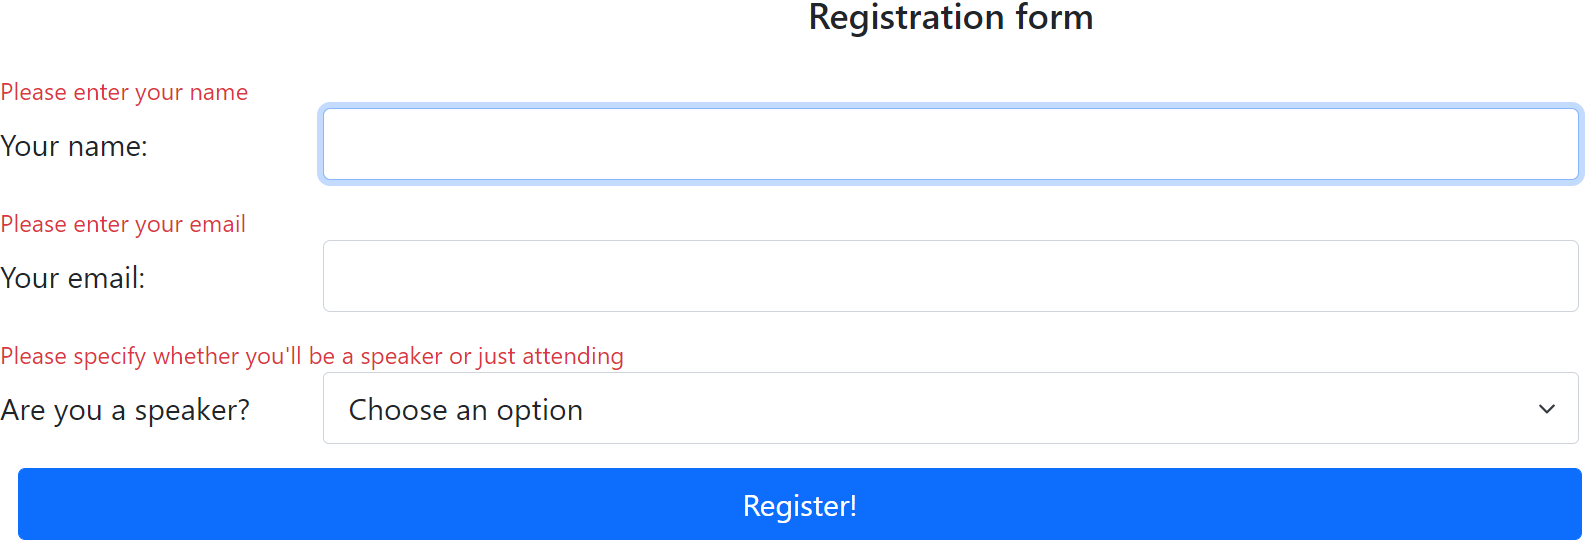
\includegraphics[width=0.8\textwidth]{validationError.png}
\end{center}

Тут мы использовали очередной тэг-хелпер, Validation Message (который выглядит как тэг span). Есть ещё Validation Summary, который печатает вообще все ошибки, найденные при валидации, но тут мы решили его не использовать.

Валидация на самом деле выполняется на сервере при Model binding-е. Если она закончилась провалом, сервер отвечает страницей, где у <<плохих>> полей формы проставлен класс, обозначающий ошибку валидации, благодаря которому и можно показать сообщение об ошибке. Но на самом деле валидацию можно силами JavaScript выполнять и на стороне клиента, и опять-таки, ASP.NET всё сделает за вас, достаточно подключить библиотеку jquery-validation, поставляемую в стандартном шаблоне:

\begin{minted}{html}
...
<head>
    <meta name="viewport" content="width=device-width" />
    <title>Register</title>
    <link rel="stylesheet" href="/lib/bootstrap/dist/css/bootstrap.css" />
    <script src="/lib/jquery/dist/jquery.js"></script>
    <script src="/lib/jquery-validation/dist/jquery.validate.js"></script>
    <script src="/lib/jquery-validation-unobtrusive/jquery.validate.unobtrusive.js" />
    </script>
</head>
...
\end{minted}

Теперь можно открыть консоль браузера (во всех нормальных браузерах это F12) и посмотреть, что при ошибке валидации сетевые запросы даже не посылаются. Что, естественно, существенно улучшает отзывчивость интерфейса и не приводит к перезагрузке страницы, то есть хорошо и правильно. Однако это не означает, что серверная валидация не нужна --- никто не мешает дёргать методы вашего веб-приложения не из его фронтенда а, например, из Fiddler, ну или, более часто, из другого веб-сервиса. Ну и вообще, у клиента может быть отключён JavaScript или он сам нагло вырезал его исполнение. Если при этом данные портятся или ваш бэкенд начинает творить что-то не то, это совсем не очень.

\section{Docker}

А теперь давайте обернём приложение в Docker-контейнер, чтобы его можно было запускать где угодно, даже там, где нет никакого .NET. Концептуально Docker --- это легковесная виртуальная машина, которая виртуализирует не машинные команды, как обычные виртуалки, а системные вызовы, то есть ядро операционной системы используется машины-хоста. Что хуже в плане изоляции, чем обычные виртуалки (например, вирусы в Docker-контейнерах запускать может быть плохой идеей), но гораздо быстрее. Ещё Docker-контейнеры отличаются от виртуалок тем, что в них работает один процесс (ну, это легко обойти, но концептуально контейнер --- это виртуализированный процесс, а не виртуализированная машина). И Docker-образы (то есть то, из чего запускаются контейнеры) только для чтения, то есть чтобы хранить в контейнере какие-то данные, надо отобразить его файловую систему на файловую систему хостовой машины. Тем не менее, Docker --- это стандарт де-факто по деплою веб-приложений, потому что позволяет запустить готовое к работе приложение буквально одной командой. 

Причём ещё есть Docker Hub, который что-то вроде GitHub для Docker-образов --- туда можно загрузить собранный Docker-образ, чтобы потом скачать на другой машине и запустить. Современные облачные провайдеры, чтобы задеплоить ваше приложение, могут попросить просто имя образа, сами укачают его с Docker Hub и запустят. Docker и Docker Hub, как и GitHub, бесплатны. Под Linux Docker поставить и настроить очень просто, под Windows, возможно, придётся повозиться --- если сделать это неправильно, он будет запускать VirtualBox, то есть настоящую виртуалку. Если сделать это правильно, придётся ставить WSL2 (к счастью, в Windows 11 она уже установлена) и терпеть исчезновение 35 Гб места на диске. И ещё, возможно, включить HyperV в настройках BIOS (который давно уже называется UEFI, но традиции сильны), но это уж как повезёт.

Итак, чтобы наше приложение запускалось в контейнере, кликаем правой кнопкой по проекту, выбираем Add Docker Support, выбираем Target OS --- Linux (даже если у вас Windows, не пугайтесь, современная Windows умеет притворяться Linux-ом) --- потому что большинство реальных хостингов работают под Linux (точнее, чем-то UNIX-подобным), и хочется, чтобы на них контейнеры работали без проблем. В проекте появится файл Dockerfile --- это конфиг сборки контейнера, типа Makefile или Docker (если вы знаете, что такое Makefile, конечно). Выглядит он примерно вот так:

\begin{minted}{docker}
FROM mcr.microsoft.com/dotnet/aspnet:6.0 AS base
WORKDIR /app
EXPOSE 80
EXPOSE 443

FROM mcr.microsoft.com/dotnet/sdk:6.0 AS build
WORKDIR /src
COPY ["ConferenceRegistration/ConferenceRegistration.csproj", "ConferenceRegistration/"]
RUN dotnet restore "ConferenceRegistration/ConferenceRegistration.csproj"
COPY . .
WORKDIR "/src/ConferenceRegistration"
RUN dotnet build "ConferenceRegistration.csproj" -c Release -o /app/build

FROM build AS publish
RUN dotnet publish "ConferenceRegistration.csproj" -c Release -o /app/publish

FROM base AS final
WORKDIR /app
COPY --from=publish /app/publish .
ENTRYPOINT ["dotnet", "ConferenceRegistration.dll"]
\end{minted}

Команда FROM задаёт, на базе какого образа строится новый образ. Docker собирает образы слоями --- при сборке поверх базового образа просто кладутся файлы и конфигурация собираемого образа. Поскольку образы read-only, это позволяет выстраивать образы в целые стеки, и при скачивании образа качать не весь его, а только те слои, которых не хватает на вашей машине. Если бы для деплоя использовались полноценные виртуалки, при каждом обновлении вашего приложения пришлось бы качать файл с виртуальной машиной, размером в несколько гигабайт. Docker в этом случае скачает только слой с вашим приложением, не перекачивая слой с инфраструктурой, это единицы мегабайт (или даже сотни килобайт) и в сотни раз быстрее.

WORKDIR --- это папка в файловой системе контейнера, которая будет рабочей для запускаемого процесса. EXPOSE открывает порт в контейнере (открываем порты 80 и 443, HTTP и HTTPS соответственно). Kestrel по умолчанию запускается на порту 5000, но базовый образ (mcr.microsoft.com/dotnet/aspnet:6.0) определяет переменные окружения, говорящие Kestrel использовать стандартные порты.

Дальше происходит самое интересное --- базовый образ сбрасывается и выполняется копирование .csproj-файла в файловую систему контейнера, дальше \emph{внутри} контейнера запускается dotnet restore, потом командой COPY . . в контейнер копируются все остальные исходники нашего проекта, и делается dotnet build. А затем (в новом слое) dotnet publish. Зачем --- чтобы даже процесс сборки не зависел от окружения. mcr.microsoft.com/dotnet/sdk:6.0 содержит .NET SDK со всеми необходимыми инструментами, так что этот Dockerfile можно будет собрать даже на машине, на которой вообще нет .NET! Если кто работал с C++, сравните это с болью, когда у вас обновился компилятор или системные библиотеки,и теперь ваш код не компилируется с дурацкими ошибками, а завтра релиз. Наш проект будет компилироваться в точно таком окружении, в котором мы его скомпилируем сейчас, до тех пор, пока Docker может найти все нужные базовые образы (возможно, даже после того, как на Земле вымрет всё живое).

Дальше базовый образ сбрасывается в base (mcr.microsoft.com/dotnet/aspnet:6.0) и в него копируется содержимое /app/publish из предыдущей фазы билда. То есть, на самом деле, создаётся чистый образ, где есть рантайм ASP.NET и бинарники нашего собранного приложения, все исходники и промежуточные результаты в финальный образ не попадают.

Ну и последняя команда --- ENTRYPOINT, определяет, что надо запускать при старте контейнера. Думаю, что тут всё понятно --- это тот самый процесс, который мы контейнеризуем.

То, что вы тут видели --- это так называемый two-stage build, то есть сначала сборка внутри контейнера, а затем запуск уже самого приложения. Это нынче модно, но, вообще говоря, опционально --- можно было собрать проект на вашей машине и командой COPY скопировать уже бинарники в образ. Приеров такого билда много в интернетах, но двухступенчатый билд лучше, и генерируется по умолчанию.

Дальше, если у вас есть Docker, можно запустить проект в Docker-контейнере через меню запуска (там, где можно выбрать хостиг и браузер). Оно соберёт образ (при этом написав в консоль, что оно делает, что приятно) и запустит контейнер из этого образа. По идее должно запуститься и работать как обычно.

А теперь давайте попробуем выложить получившийся образ на Docker Hub. Для этого там, естественно, надо завести аккаунт. Далее, кликаем правой кнопкой по проекту, выбираем Publish, выбираем Docker Container Registry, Docker Hub, вводим свои логин-пароль, жмём Publish. Оно снова соберёт образ и, по идее, зальёт его на Docker Hub. Но может и не зальёт, там какие-то проблемы с <<Current context "desktop-linux" is not found on the file system>>. Но это не беда, Docker вообще по сути своей консольная утилита. Идём в консоль, набираем там docker images ls (отобразить спискок всех образов, что есть на машине), находим наш (например, conferenceregistration latest 2fdfa15fbf59 10 minutes ago 239MB). Сначала его надо переименовать в формат <имя пользователя>/<имя образа>, чтобы Docker Hub разрешил вам его пушить:

\begin{minted}{text}
docker image tag conferenceregistration:latest 
    <ваш юзернейм на Docker Hub>/conferenceregistration:latest
\end{minted}

(в одну строчку). Дальше, собственно, пушим на Docker Hub (перед этим по идее надо авторизоваться через Docker Desktop, но могут и при пуше попросить логин/пароль, я не помню):

\begin{minted}{text}
docker push <ваш юзернейм на Docker Hub>/conferenceregistration:latest
\end{minted}

И всё, через некоторое время образ зальётся, можно зайти на Docker Hub и проверить, что образ появился. Теперь вы можете пойти на другую машину, где есть Docker (например, одногруппника) и скачать/запустить ваш образ:

\begin{minted}{text}
docker run -d -p 80:80 <ваш юзернейм на Docker Hub>/conferenceregistration:latest
\end{minted}

Теперь можно просто в адресной строке браузера набрать localhost, и попасть в наше приложение (либо в Docker Desktop найти запущенный контейнер, посмотреть его логи и нажать на <<открыть в браузере>>). Собственно ключ -p у команды docker run прокидывает порт 80 контейнера на 80 порт вашей машины (а ключ -d (detach) говорит, что надо вернуть управление в консоль после старта контейнера). Прокидывание портов делается при запуске, чтобы если у вас на машине надо запустить 20 контейнеров, каждый из которых работает на порту 80, вы могли бы их раскидать сами по портам, не пересобирая контейнер.

\section{Azure}

И наконец, выложим наше барахло на облачный хостинг, в нашем случае на Azure (вообще, Amazon был бы выбором по умолчанию, но раз уж .NET, надо уважать Microsoft). 

Идём на \url{https://azure.microsoft.com/} и регистрируем себе аккаунт. Дальше логинимся и идём на \url{https://portal.azure.com/}. Выбираете там App Services -> Create. В появившейся форме выбираете Pay-As-You-Go, Resource Group -> Create New, вводите имя группы ресурсов. Ниже вводите имя приложения, например, conference-registration, оно же будет частью его доменного имени. Publish --- Docker Container, Operating System --- Linux (мы ведь собирали линуксовый образ), Region --- например, East US (от региона зависит физическое местонахождение сервера, и, главное, доступные ценовые планы), App Service Plan --- создастся новый по идее сам, Sku and size --- бесплатный (F1 вроде) --- невероятно медленно и плохо, но бесплатно. Жмём next.

Дальше выбираем Single container, Image Source -> Docker Hub, Access Type -> Public, Image and Tag --- имя образа на Docker Hub, тот самый <ваш юзернейм на Docker Hub>/conferenceregistration:latest), и этого достаточно. Жмём на Review + create. Жмём на create. Оно некоторое (долгое, мы ведь нищеброды) время думает и показывает Deployment is in progress, после чего появляется Your deployment is complete, и можно пойти на домашнюю страницу, там наше приложение появится в списке ресурсов. Жмём на него, появляются детали приложения, жмём на Browse, и приложение начнёт медленно открываться в браузере (по ссылке в духе \url{https://conference-registration.azurewebsites.net/}). Всё, приложение запустилось, теперь эту ссылку можно использовать, чтобы зайти на него вообще откуда угодно, хоть с телефона. 

Этот радостный факт и завершает этот туториал.

\end{document}
